% !TEX root =  ../supplementary.tex

\section{Demonstration of Personalized Schedules for Patient 911 and Patient 2340}
\label{sec : demo_911_2340}

In this section we demonstrate the application of personalized schedules on patients from PRIAS. In Section \ref{subsec : demo_prias_pers_schedule} of the main manuscript we demonstrated personalized schedules for patient 3174. Here we demonstrate them for the remaining two patients.

The second patient of the demonstration data set is patient 911, for whom the evolution of PSA, time of last biopsy and proposed biopsy times are shown in the top panel of Web Figure \ref{web_fig : prias_demo_pid_911}. We can see the combined effect of decreasing PSA levels and a negative repeat biopsy on personalized schedules, between year three and year 4.5 for this patient. In accordance with the many negative repeat biopsies and consistently decreasing PSA, the proposed time of biopsy based on expected time of GR increases from 16.6 years to 18.8 years in this period. We can also see that after each repeat biopsy, $\mbox{SD}[T^*_j] = \sqrt{\mbox{var}_g(T^*_j)}$ decreases sharply (bottom panel of Web Figure \ref{web_fig : prias_demo_pid_911}), thus in turn reducing the offset as well. As for schedules based on dynamic risk of GR, in accordance with the many negative repeat biopsies and consistently decreasing PSA, the proposed time of biopsy increases from 14 years to 15 years during the time period of interest.

\begin{figure}
\centerline{
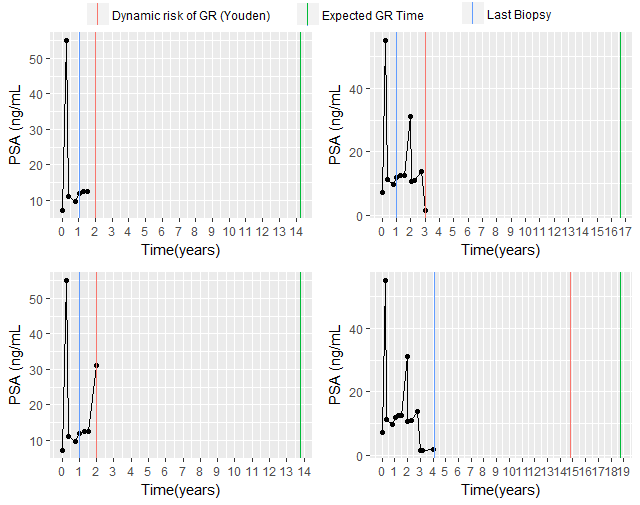
\includegraphics[width=\columnwidth]{images/prias_demo/case_911.png}
}
\caption{Top panel: Evolution of PSA, history of repeat biopsies and corresponding personalized schedules for patient 911. Bottom Panel: History of repeat biopsies and $\mbox{SD}_g(T^*_j) = \sqrt{\mbox{var}_g(T^*_j)}$ over time for patient 911.}
\label{web_fig : prias_demo_pid_911}
\end{figure}

Patient 2340 presents a case where information from PSA levels and repeat biopsies is conflicting. In Web Figure \ref{web_fig : prias_demo_pid_2340} we can see that the PSA for this patient becomes twice between year two and year 3.2. If only information from PSA is considered, then we can see that proposed time of biopsy based on expected time of GR is preponed from 14.6 to 13.0 years during this period. However, if we also take into account the negative result from the repeat biopsy at year 2.5, then the proposed time of biopsy is postponed from 14.6 years to 15 years. Thus more weight is given to a recent negative biopsy result than PSA, which is in accordance with the clinical practice. The proposed time of biopsy based on dynamic risk of GR is also postponed from 2.3 to 3.6 years in light of the negative biopsy result.

\begin{figure}
\centerline{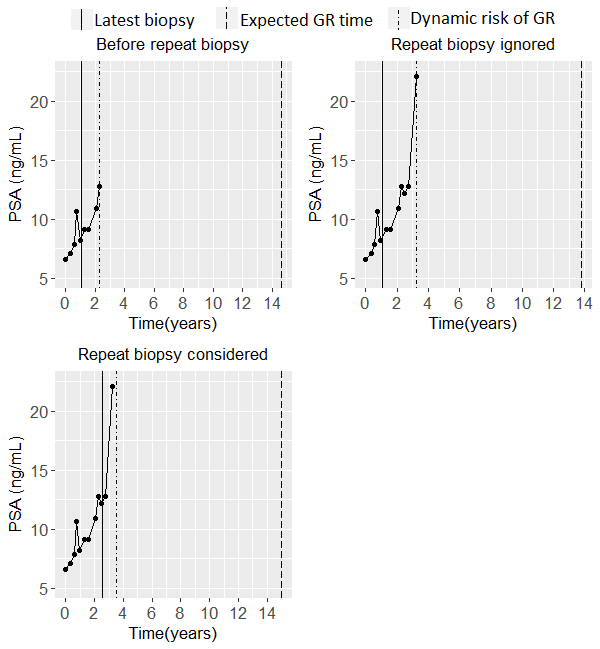
\includegraphics[width=\columnwidth]{images/prias_demo/case_2340.png}}
\caption{Evolution of PSA, history of repeat biopsies and corresponding personalized schedules for patient 2340.}
\label{web_fig : prias_demo_pid_2340}
\end{figure}